\chapter{Design}
The TEBNF language makes it possible to convert a software design expressed as a state machine and convert it into a specification that can be provided to the TEBNF code generation tool.  The TEBNF code generation tool generates C++ 11 code from TEBNF grammars that can be built by a C++ compiler into a functioning console application.  This chapter discusses the TEBNF language, design decisions, the TEBNF code generation tool, the architecture of the tool, and the code generation process.

\section{The TEBNF Language}
The TEBNF specification is composed of language constructs called elements.  A TEBNF grammar is the combination of these elements and their contents to define an application.   The primary function of each element type is to convey one specific functionality.  One advantage of this approach is scalability.  The complexity of each element is reduced because each element does one thing only.  This follows the established design paradigm of making something do only one thing but do it well.  There are five kinds of elements in the TEBNF specification:
\begin{itemize}
  \item Input methods: a method of receiving data as input.
  \item Output methods: a method of outputting data.
  \item Grammar sections: parses input data. 
  \item Actions: action code to execute using data from other elements.
  \item State transition tables: defines execution path.
\end{itemize}

\indent
Within each element are separate constructs known as subelements.  Different kinds of subelements exist for each element type, and are enumerated in detail in appendix~\ref{appendix:TEBNF}.  The glue that brings these elements together to describe an application is two-fold: 1) static variables that can be defined within grammar elements and used by other elements to get and store information, and 2) state transition table elements that use all of the other elements in a grammar to express the order of task execution.

\subsection{Design Decision: Singleton Paradigm}
One of the primary goals of TEBNF is to reduce the difficulty of translating high-level designs into grammars.  Keeping TEBNF simple means that developers are spending more time designing how an application will be used rather than worrying about many of the details associated with translating their design into code.   Elements have been designed to behave as singletons in TEBNF, as well as the code generated from them.

\indent
Multiple reasons and advantages exist for treating TEBNF elements and the C++ classes generated from them as singletons:
\begin{itemize}
  \item Lazy instantiation.  Singleton C++ classes make it possible to avoid allocating memory for element class objects until they are actually used in the generated code.  This is different from static initialization that allocates memory to a variable at the time of declaration.
  \item Thread synchronization.   Singletons can yield the best results in situations where multiple threads try to access the same resource.  This applies to code generated from a TEBNF grammar because it is possible for multiple state table threads to need access to the same subelement or static variable class members at the same time.
  \item Instance control.  A singleton prevents other objects from instantiating their own copies of the singleton object, ensuring that all objects access the same instance.  This simplifies the design process in TEBNF because grammar writers know exactly what they are accessing in their grammar.
  \item Flexibility.  Generated singleton element classes control the instantiation process.  This control over the instantiation process gives them the flexibility to change the process.  Since TEBNF purposely abstracts these details from grammar writers, it is advantageous for each element class to control the way it is instantiated based on how it is used/interacts in the generated application code.
\end{itemize}

\subsection{Design Decision: Adapting TEBNF}
Some complexities in the TEBNF language were exposed as the code generation tool was written.  When encountered, adaptations to TEBNF were made to better represent their nature and interaction of these complexities within the language.  Design decisions made with respect to TEBNF elements are discussed in~\ref{ssec:IoElements} and~\ref{ssec:ActionsElements}.

\subsection{Design Decision: Input and Output Elements} \label{ssec:IoElements}
Console applications typically get string or numerical input from users by displaying questions and waiting for the user to type an answer.  Attempting to determine the type of input information in generated code could lead to incorrect interpretations of the input type at run time.  One technique that was considered to avoid this problem is to directly tie grammar subelements or static variables to input subelements.  This method proved to be unwieldy because grammar elements change during the natural process of writing a TEBNF grammar.  Simply changing the name of a grammar subelement would require that name to be changed in every input subelement tied to it.  This problem could be compounded as other input elements are created that contain subelements tied to the same grammar subelements or static variables.   To resolve this problem, console input subelements tie each question string to a type (appendix~\ref{appendix:TEBNF}).  The responsibility of knowing the expected input type falls to the grammar writer rather than a risky prediction.

\indent
Usage of console output elements in TEBNF was found to be simpler than console input.  This is due to the fact that generated console output code performs a simple passing of output data to a C++ std::cout statement.   Because std::cout easily handles outputting of numerical and string data, there is no need for special handling in TEBNF.

\indent
Support for sending and receiving data over UDP is achieved in TEBNF using UDP elements.  The TEBNF language uses UDP I/O elements to abstract most of the details involved with setting up and using UDP sockets.  Generated UDP I/O element classes prompt users for an IP address and port number before initiating UDP communication.  It became apparent that a way was needed to indicate that a UDP output element should send data on the same socket instance used by an existing UDP input element to receive data.  The "“AS"” keyword expresses this relationship between two I/O elements of the same type.  The “"AS"” relationship defines an element that shares all of the same characteristics as another I/O element of the same type.  Because TEBNF elements and their respective C++ element classes are singletons, all that is needed to represent this case in generated C++ code is a type definition of the I/O element in question (typedef).  This reduces the number of C++ classes generated.

\subsection{Design Decision: Actions Elements} \label{ssec:ActionsElements}
Actions elements in TEBNF share two similarities to C++ functions. The first similarity is the ability to have one or more parameters, allowing arguments to be passed inside state transition table elements.  Second, actions elements can contain multiple instructions.  Actions elements also allow grammar writers to access subelements and/or static variables found in any grammar element.  The syntax for accessing subelements defined inside other grammar elements can be found in appendix~\ref{appendix:TEBNF}.

\indent
Unlike C++ functions, actions elements cannot return values.  TEBNF purposely abstracts this kind of complexity from grammar writers.  This kind of functionality was intended to be expressed in state transition table elements.  In TEBNF, a “return value” is expressed in a state transition table when a state'’s input or condition criteria is met, resulting in data being routed (returned) to an output and/or optionally transitioning to a different state.  This supports their intended usage as the action(s) component of one or more states in a state machine.  A side effect of actions elements not returning values is that they cannot be used as the input or condition of a state within a state transition table element.  This is due to the fact that the resulting type of a state’s input or condition must be a Boolean.  This also illustrates one of the ways that TEBNF abstracts complexity through state machine design.

\indent
Actions elements are essentially C++ code blocks that allow direct reference to TEBNF subelements and static variables.  This means they have loose parsing requirements compared to other TEBNF elements so that the chosen C++ compiler can catch complex errors in actions element code.

\section{The TEBNF Code Generation Tool}
This report presents a prototype code generation tool that generates the lexical analysis, parsing, and actions code of a basic console application using a single TEBNF grammar as input.  Generated applications accept user input where necessary and can provide meaningful status.  The tool outputs a set of classes that:
\begin{enumerate}
  \item Accept input data through console, file, or UDP/IP.
  \item Provide a set of functions that unmarshal raw data into human-readable types such as numbers and strings, and can marshal it back into its original form.
  \item Use these unmarshal functions to match input data to pattern(s) specified in the grammar and convert them to human-readable values.
  \item Run one or more state machines with each on its own thread to receive data through input methods described in the grammar.  As input data arrives, the state machine finds matches to grammar patterns and executes actions that produce the desired output.
  \item Provide a console-based user interface that prompts for input as needed and provides status.
\end{enumerate}

\indent
The architecture of the TEBNF code generation tool consists of four stages, shown in figure~\ref{fig:TEBNFCodeGenToolArchitecture}.  The TEBNF code generation tool is a console application that accepts three arguments in order:
\begin{enumerate}
  \item Path of the file containing a TEBNF grammar.
  \item Path of directory where the tool will write generated code.
  \item The name to give to the generated application.
\end{enumerate}

\begin{figure}[h!]
\centering
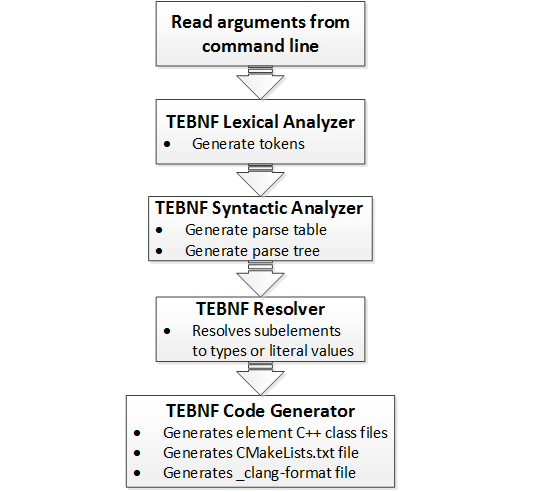
\includegraphics[width=0.9\textwidth]{figures/TEBNFCodeGenToolArchitecture.png}
\caption{Architecture of the TEBNF prototype code generation tool.}
\label{fig:TEBNFCodeGenToolArchitecture}
\end{figure}

\indent
Upon receiving these arguments, the tool reads the grammar file at the location provided to the tool.  The grammar is lexically analyzed by the TEBNF scanner to produce a list of tokens, with some metadata attached to some tokens as needed.

\indent
The TEBNF parser syntactically analyzes these tokens using a recursive descent algorithm to verify correctness of format.  A pointer to each element discovered by the parser is then added to a table for quick look up and inserted into a parse tree.  Subelements discovered during this parsing stage are added to their parent elements and subelements as they are found in the parse table and parse tree.

\indent
After all of the elements and subelements have been added to the parse table and parse tree, the TEBNF resolver traverses the subelements in the parse tree and their descendants to their furthest extent (leaves).  This ensures that all subelements resolve to a terminal type or literal value.

\indent
After all elements and their subelements have been resolved, the TEBNF code generator iterates through each element in order of declaration in the input grammar, and generates a C++ class or other appropriate C++ code.  The name of each C++ source file corresponds to the element it was generated from.  A CMakeLists.txt file is generated with these C++ source files so that CMake can be used to generate Microsoft Visual Studio 2013 solution and project files.  For convenience, a \_clang-format file is generated so that any clang-formatting (optional) follows the intended format.

\section{Lexical Analysis and Parsing Code Generation}
The TEBNF code generation tool generates a class for each input/output (I/O) element (method) defined in a TEBNF grammar (see appendix~\ref{appendix:TEBNF}).  These I/O classes perform no lexical analysis.  They only receive input and/or send output.  Supported I/O methods are as follows:
\begin{itemize}
  \item Console
  \item File
  \item UDP/IP
\end{itemize}

\indent
These I/O methods are a powerful feature of TEBNF and the TEBNF code generation tool because the tool automatically integrates the code to do I/O using these methods.  The complexities of their usage are abstracted by the tool, which is one of the key advantages of TEBNF and the TEBNF code generation tool.  Contrast this to the most common code generation tools, which do not provide this built-in I/O capability.

\indent
Lexical analysis and parsing is performed by the generated code in one step rather than separate steps.  This is possible because of the way patterns are described in TEBNF grammar elements (see appendix~\ref{appendix:TEBNF}).  A typical grammar element pattern is composed of groupings of bytes broken into sub-groupings of bytes.  These sub-groupings can be translated into specific types (e.g. numbers, and strings) and literal values.  The size in bits or bytes is defined in the grammar element based on its type.

\indent
Matching user-defined TEBNF grammar patterns to incoming data requires that one or more literal values be defined somewhere in the grammar.  The value of a literal value makes it possible to find it in the input data.  The size and type of that initial literal value is defined implicitly or explicitly in the grammar (e.g. 4-byte integer, etc.).  Given the initial reference offset $ \alpha_f $ of the literal $ f $ and its size $ z_f $, the offset of the literal or type immediately following it is defined as $ \alpha_{f+1} $, where $ \alpha_{f+1} = \alpha_f + z_f $.  The offset of the literal or type defined immediately before $ f $ can be defined as $ \alpha_{f-1} $, where $ \alpha_{f-1} = \alpha_f {-} z_{f-1} $ and $ z_{f-1} \geq \alpha_f $.  The data offsets of subsequent literals and/or types found before and after the initial reference offset are calculated based on the one after and before it, respectively.

\indent
When multiple patterns must be matched to incoming data, a separate grammar element must be written to describe each pattern.  This design makes it possible to refer to any given pattern using its grammar element name, making it easy to distinguish from other grammar patterns in the same TEBNF grammar.

\begin{figure}[htbp]
\centering
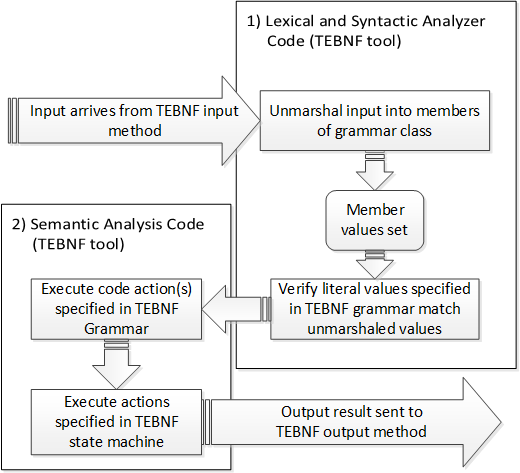
\includegraphics[width=0.9\textwidth]{figures/GeneratedCodeExecutionPath.png}
\caption{Execution path for code generated by the TEBNF code generation tool.}
\label{fig:GeneratedCodeExecutionPath}
\end{figure}

\indent
Grammar elements are translated by the prototype code generation tool into classes that serve a three-fold purpose.  Each grammar class can (1) unmarshal raw input data into specific user-defined types, (2) verify matches to byte patterns in the raw input data, and (3) marshal the values stored in the grammar class back into their original form and byte ordering.  Patterns in data arriving through TEBNF input methods are located by the state machine using unmarshal functions of grammar element classes.  As data arrives through an input method, patterns are recognized in the data by the grammar classes and simultaneously unmarshaled into the data types of those classes.  This means lexical analysis and parsing are performed in the same step, using a single TEBNF input (figure~\ref{fig:GeneratedCodeExecutionPath}).  This approach is different from traditional parser code generation methods.  Traditional methods require the use of a lexical analyzer generator tool and parser generator tool; each with their own input specification formats (see figure~\ref{fig:TraditionalCodeGenProcess}).

\section{State Machine and Actions Code Generation}
Path(s) of execution are defined in TEBNF using state machines, as shown in figure~\ref{fig:GeneratedCodeExecutionPath}.  State machines are represented in TEBNF using state transition table elements (see appendix~\ref{appendix:TEBNF}).  A state machine in TEBNF describes the order of tasks executed by a single application thread.  States are divided into a series of six steps.  These six steps are given below, in the order they are expressed in TEBNF, which is the same order they are evaluated by the generated code:
\begin{enumerate}
  \item A unique name that identifies the state and allows other states to reference it
  \item A Boolean condition that can be either a grammar to match with input data, or an explicit Boolean condition.
  \item The method of input for receiving the input data (console, file, or UDP/IP).
  \item The next state to jump to if the Boolean condition provided in the second step evaluates to true.
  \item An output or action to send through the output method provided in the sixth step.
  \item The method of output to send through the output method provided in the fifth step, or an explicit code action to execute.
\end{enumerate}

\indent
These state steps shape the way TEBNF elements interact with each other and input data by determining (1) what input methods data is received on, (2) what parts of the received data match defined grammar patterns, (3) what method is used to output that data, and (4) what code actions are executed.
